\documentclass{sigchi}

% Use this command to override the default ACM copyright statement (e.g. for preprints). 
% Consult the conference website for the camera-ready copyright statement.


%% EXAMPLE BEGIN -- HOW TO OVERRIDE THE DEFAULT COPYRIGHT STRIP -- (July 22, 2013 - Paul Baumann)
% \toappear{Permission to make digital or hard copies of all or part of this work for personal or classroom use is 	granted without fee provided that copies are not made or distributed for profit or commercial advantage and that copies bear this notice and the full citation on the first page. Copyrights for components of this work owned by others than ACM must be honored. Abstracting with credit is permitted. To copy otherwise, or republish, to post on servers or to redistribute to lists, requires prior specific permission and/or a fee. Request permissions from permissions@acm.org. \\
% {\emph{CHI'14}}, April 26--May 1, 2014, Toronto, Canada. \\
% Copyright \copyright~2014 ACM ISBN/14/04...\$15.00. \\
% DOI string from ACM form confirmation}
%% EXAMPLE END -- HOW TO OVERRIDE THE DEFAULT COPYRIGHT STRIP -- (July 22, 2013 - Paul Baumann)


% Arabic page numbers for submission. 
% Remove this line to eliminate page numbers for the camera ready copy
% \pagenumbering{arabic}


% Load basic packages
\usepackage{balance}  % to better equalize the last page
\usepackage{graphics} % for EPS, load graphicx instead
\usepackage{times}    % comment if you want LaTeX's default font
\usepackage{url}      % llt: nicely formatted URLs
\usepackage{listings}

% llt: Define a global style for URLs, rather that the default one
\makeatletter
\def\url@leostyle{%
  \@ifundefined{selectfont}{\def\UrlFont{\sf}}{\def\UrlFont{\small\bf\ttfamily}}}
\makeatother
\urlstyle{leo}


% To make various LaTeX processors do the right thing with page size.
\def\pprw{8.5in}
\def\pprh{11in}
\special{papersize=\pprw,\pprh}
\setlength{\paperwidth}{\pprw}
\setlength{\paperheight}{\pprh}
\setlength{\pdfpagewidth}{\pprw}
\setlength{\pdfpageheight}{\pprh}

% Make sure hyperref comes last of your loaded packages, 
% to give it a fighting chance of not being over-written, 
% since its job is to redefine many LaTeX commands.
\usepackage[pdftex]{hyperref}
\hypersetup{
pdftitle={Follow-focus with Arduino},
pdfauthor={LMU Munich},
pdfkeywords={SIGCHI, proceedings, archival format},
bookmarksnumbered,
pdfstartview={FitH},
colorlinks,
citecolor=black,
filecolor=black,
linkcolor=black,
urlcolor=black,
breaklinks=true,
}

% create a shortcut to typeset table headings
\newcommand\tabhead[1]{\small\textbf{#1}}


% End of preamble. Here it comes the document.
\begin{document}

\title{Follow-focus with Arduino}

\numberofauthors{3}
\author{
  \alignauthor Christian Guerrero\\
    \affaddr{Ludwig Maximilian Universit\"at, M\"unchen, Munich, Germany}\\
    \email{christian.guerrero@campus.lmu.de}\\
  \alignauthor Arthur Moufounda\\
    \affaddr{\'{E}cole Sup\'{e}rieure Des Technologies Industrielles Avanc\'{e}es, Bidart, France}\\
    \email{a.moufounda@net.estia.fr}\\
  \alignauthor Alexander Schenker\\
    \affaddr{Ludwig Maximilian Universit\"at, M\"unchen, Munich, Germany}\\
    \email{alexander.schenker@campus.lmu.de}\\
}

\maketitle

\begin{abstract}

\end{abstract}

\keywords{
	Guides; instructions; author's kit; conference publications;
	keywords should be separated by a semi-colon. \newline
}

\section{Motivation and Background}

\subsection{General Motivation}
In the field of cinema for instance, we success to semi-automatized the travelling. What we want to do is doing the same with the focus pulling, using the follow focus.

Normally, manual control is required in order to zoom and to keep the focus on the desired object. In classical productions, the focus puller (or first Assistant Camera) is a dedicated position, whose job it is to keep the focus, according to the cinematographers instructions. As there is no way to correct a falsely set focus in post-production, it is considered one of the hardest jobs on a film set. So, the solution would be to create a super-precise way of focusing an object, which would excluded a possible human error.
By using a wireless motion controller and setting different sequences of movement then remembering it, the result would be extremely precise and repetable ; another advantage would also be that the movement would fluider, with a direct speed control and linearity.
That what’s we aim in our project. Combined with the precedent travelling work, it would permit to create a follow focus of an object, keeping the best focal distance each second, without direct manual interaction with the camera.
This project could have utility in application such recording scenes in an impracticable environment for a human for instance.


\subsubsection{General Description of the Topic}

\subsubsection{State of the Art in Follow Focus}

So, which technology are used in the field of follow focus ?
Andrea Motion Focus
First, we can speak about the Andra Motion Focus. This company developed a follow system with a very high accuracy. Using a portable and easy to set up magnetic mo-cap system, it’s able to very accurately track subjects and cameras in real time and use that data to drive a lens control motor.  The mo-cap side of the system uses very small sensors which can be mounted to the performer beneath clothing, just like a lavalier microphone. The user can then decide where they want the focal point, relative to that sensor, and the system does the rest. 
There are two ways to interface with the system. The basic approach to use an iPad. Another option is to use the hand unit (The Arc).
The system can also be used to “save” positions of non moving objects in any given area, and, for dyed in the wool focus pullers who want to do it all manually, the hand unit streams live distance data of any chosen subject or object whether it’s moving or stationary.  You can choose to let the system pull focus for you, allowing you to simply decide when and how fast to move between subjects, or you can just use the data to pull manually.

Show Focus

Designed to facilitate the duties of the on-set focus-puller, Show-Focus renders a physical representation of the invisible plane of focus so that the precise focal point can be deduced, and captured, at any time. The model is compromised of two components, communicable through a wireless connection: the camera module and the controller. The camera module, which is attached to the body of the shooting camera, provides a real-time 3D map of what is being filmed, while also controlling the focus ring through a motorized mechanism. The controller — as its name suggests — displays the map and allows the focus-puller to oversee the movements of the focus ring.

PROAIM Camera Follow Focus X1 (FF-X1)

On the market, you can find a lot of product like this one. Using gear driven designed, the FF-X1 ensures smooth accurate emphasis over your subject. Designed to give slip-free, accurate and repeatable focus movement on a wide range of cameras are possible.


\subsection{Background}

\subsubsection{Vision}

\subsubsection{Current Research at LMU}

\section{Solution}

\subsection{Our Follow Focus Approach}
Our solution is based on the ideas of \textit{DIY Follow Focus} and \textit{Soffer Follow Focus}.

What we want is a device adaptable to all types of camera. We also want a remote controller, which will work as interface between user and camera. A step motor attached to a gear would ensure the focus pulling depending on the received signal from the remote controller.
Now those are the functionalities we want to implement:
\begin{itemize}
  \item Real time focus pulling (in and out).
  \item The speed of focus change should be adjustable.
  \item The camera's range should be configurable.
  \item We want to be able to record several motion sequences and play them back.
\end{itemize}

\subsection{Methods}
To realize our aims we decided to develop an Arduino App for input. It sends via Bluetooth a perpetual signal to a BTLE module connected to an Arduino Nano. The Arduino processes those bytes and sends commands to a StepperDriver connected to a AccelStepper. 


\subsubsection{Electrical Engineering}
Top of all, we wanted our follow focus to be portable. Therefor the elements had to be small, low energy powered and easily embeddable. These challenges had to be tackled in the planning phase of the process. So at first we had to decide between different technologies in order to meet our aims:
\begin{itemize}
\item The remote controller would be a smart phone. Thus, anyone could easily control the follow focus device by downloading our application in the app store.
\begin{figure}
	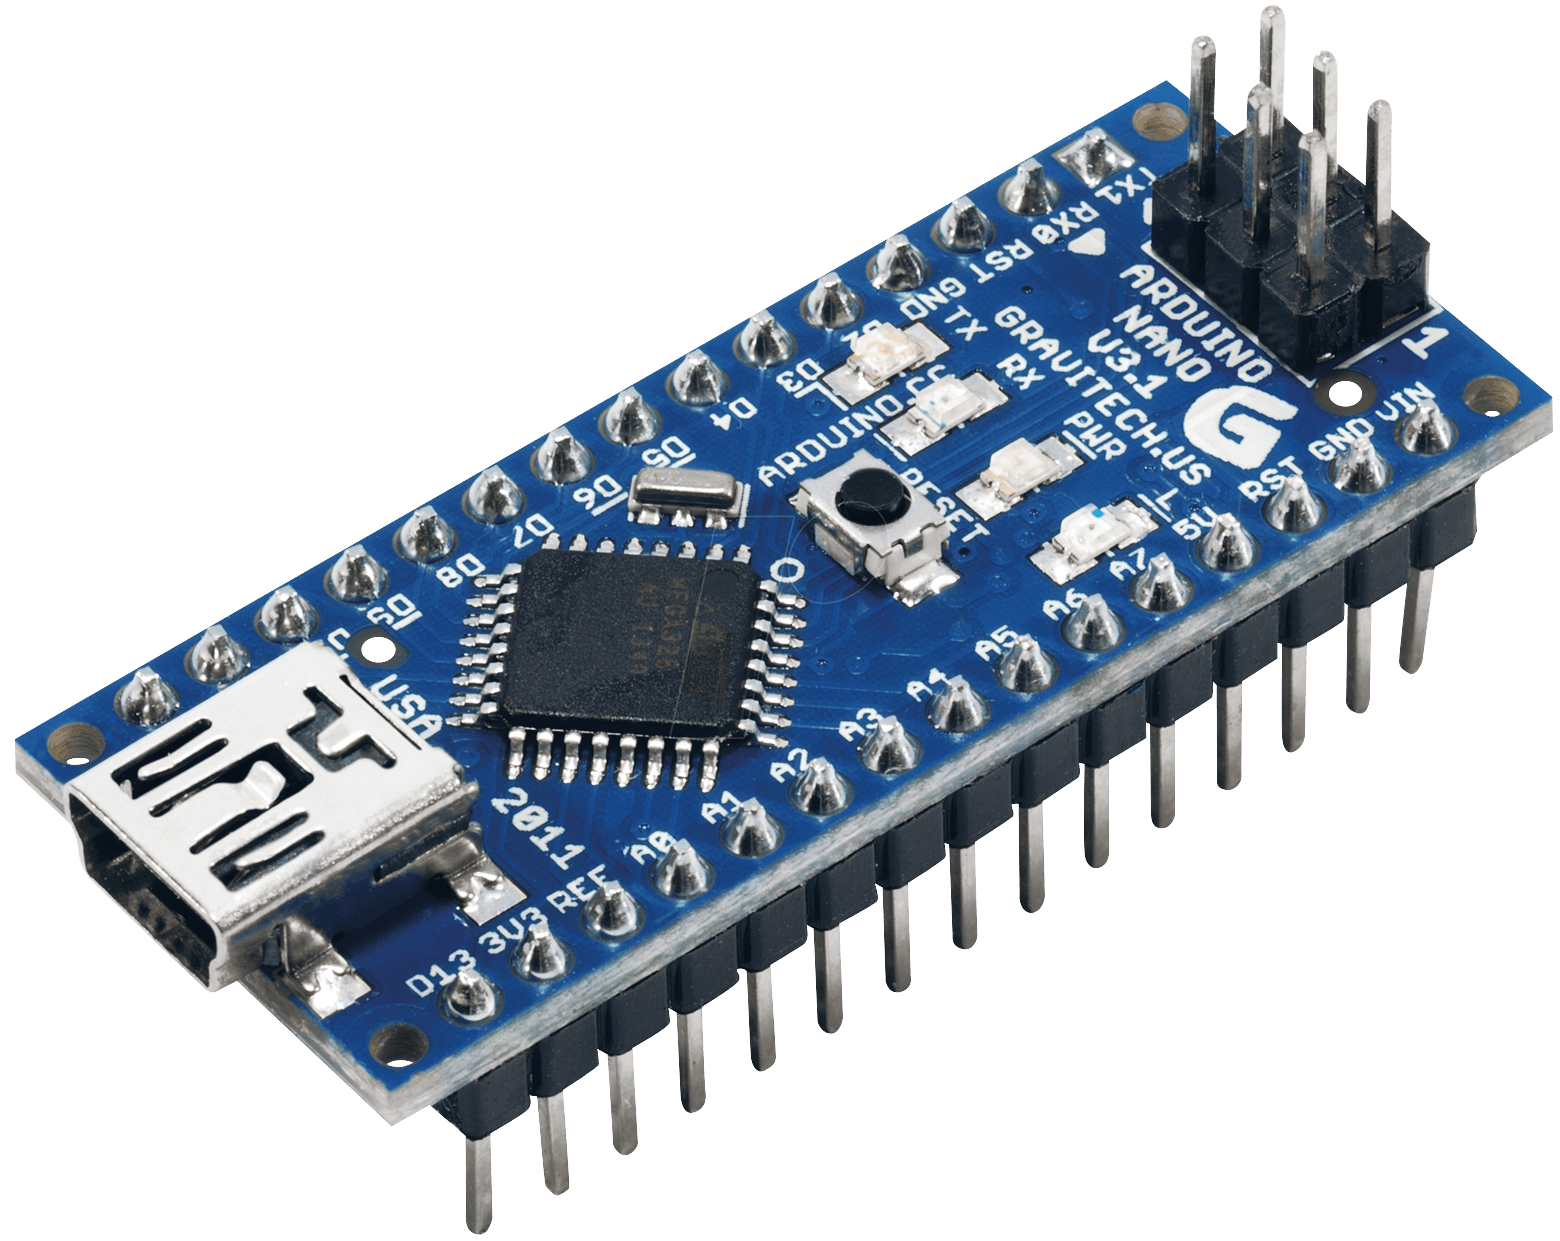
\includegraphics[width=0.4\textwidth]{nano.png}
\end{figure} 
\item For our requirements an Arduino Nano is more than sufficient. It is small and consumes only little.
\begin{figure}
	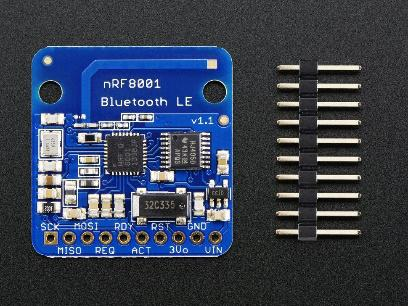
\includegraphics[width=0.4\textwidth]{btle.jpg}
\end{figure} 
\item For the Wireless control we use Bluetooth LE because of its low energy, easy implementation and also because there is a large web community and many examples available online.
\begin{figure}
	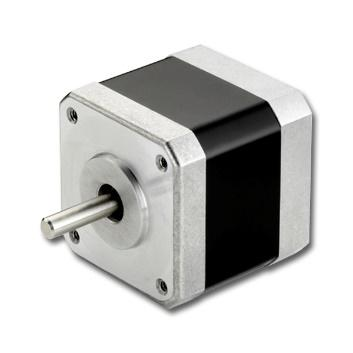
\includegraphics[width=0.4\textwidth]{stepper.jpg}
\end{figure} 
\item A stepper motor is used because it works more precise and faster than a servo and has only small enertia. Also with stepper we always know the exact amount of rotation we have to apply.
\begin{figure}
	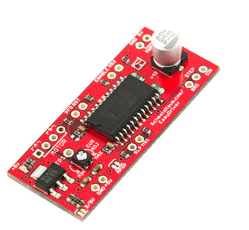
\includegraphics[width=0.4\textwidth]{driver.png}
\end{figure} 
\item Having a motor is good. Adapting it to an electrical system is better. The stepper driver will protect the Arduino Nano from different electrical damages that may be caused by the sudden increase of intensity caused by the motor. It also allows to turn in both directions.
\item The AccelStepper library for Arduino is very useful as it makes the API never to block and supports very slow speeds. Also it helps to easily apply acceleration.
\item None of the electronic parts is passive. To make them all work, we need electric energy, but we also want our global system to be portable. Therefor we will use different sets of battery, because the Arduino and the step motor need to be powered separately, at least 5V and 12V respectively.
\end{itemize}
In the attached code of the Arduino we see how the components work together.
\begin{lstlisting}
if (status == ACI_EVT_CONNECTED) 
  {
    stepper.enableOutputs();
    stepper.run();
    if (BTLEserial.available()>0) 
    {
      digitalWrite (enablePin, LOW);
      previousMillis = millis();
      dataReceive = BTLEserial.read();
      react(); //function to react to input   
      stepper.run();
      stepper.moveTo(encoderValue);
    } 
	...

void react()
{
  if (dataReceive > 48 && dataReceive < 58)  //[1-9]-Key
  {
    speedValue = map(dataReceive, 49, 57,
    	minSpeedValue, maxSpeedValue);
    stepper.setMaxSpeed(speedValue);
    Serial.println(speedValue);
  } 
  else if (dataReceive == 43) //[+]-Key
  {
    encoderValue += stepSize;
  }
  else if (dataReceive == 45)  //[-]-Key
  {
    encoderValue -= stepSize;
  }    
  else if (dataReceive == 0) {
    encoderValue = stepper.currentPosition();
  }
  ...
\end{lstlisting}

 
\subsubsection{Case Modeling}
\begin{figure}
	\center
	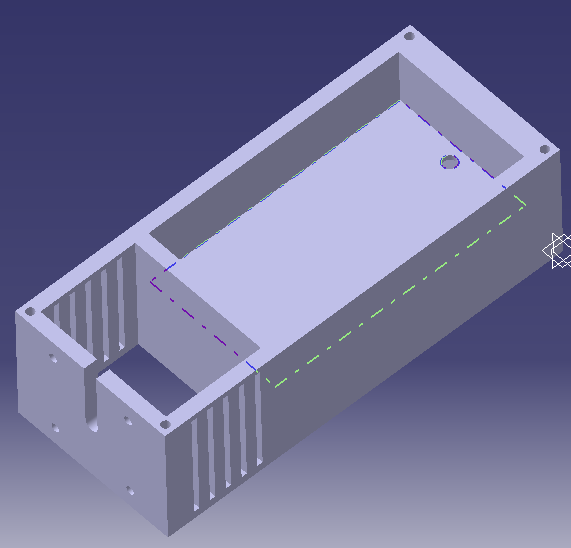
\includegraphics[width=0.4\textwidth]{case.png}
\end{figure} 
For building our case we faced two questions. Which size and which technology - 3D-printing or laser cutting. First we designed the parts with CATIA, the 3D modeling software from Dassault System. But the 3D-model took a lot of printing time and in the end they felt very unstable. So we used laser cutting on 3mm wood in the end which is to a very nice looking and useful material. Also for redesigning and resizing this easy manipulative material proved to be best.
The box is composed of three compartments. The first part is the place which houses the electronic parts. A similar space exists underneath and is designed for the batteries, to allow exclusive access. The back of the case has two nicks which allow to open the backside easily when a battery exchange is due. In the front of the box is a place for the stepper motor, which can be screwed in. The notches on the sides are supposed to evacuate the heat produced by the motor when it is at work. Two holes drilled into the partition walls allow wires to connect the Arduino, stepper and battery compartments.



\subsubsection{App Development}

\section{Discussion \& Next Steps}

\section{Conclusion}

\bibliographystyle{acm-sigchi}
\bibliography{sample}
\end{document}
